%%%%%%%%%%%%%%%%%%%%%%%%%%%%%%%%%%%%%%%%%%%%%%%%%%%%%%%%%%%%%%%%%%%%%%
% LaTeX Example: Project Report
%
% Source: http://www.howtotex.com
%
% Feel free to distribute this example, but please keep the referral
% to howtotex.com
% Date: March 2011 
% 
%%%%%%%%%%%%%%%%%%%%%%%%%%%%%%%%%%%%%%%%%%%%%%%%%%%%%%%%%%%%%%%%%%%%%%
% How to use writeLaTeX: 
%
% You edit the source code here on the left, and the preview on the
% right shows you the result within a few seconds.
%
% Bookmark this page and share the URL with your co-authors. They can
% edit at the same time!
%
% You can upload figures, bibliographies, custom classes and
% styles using the files menu.
%
% If you're new to LaTeX, the wikibook is a great place to start:
% http://en.wikibooks.org/wiki/LaTeX
%
%%%%%%%%%%%%%%%%%%%%%%%%%%%%%%%%%%%%%%%%%%%%%%%%%%%%%%%%%%%%%%%%%%%%%%
% Edit the title below to update the display in My Documents
%\title{Project Report}
%
%%% Preamble
\documentclass[paper=a4, fontsize=11pt]{scrartcl}
\usepackage[T1]{fontenc}
\usepackage{fourier}

\usepackage[english]{babel}															
% English language/hyphenation
\usepackage[protrusion=true,expansion=true]{microtype}	
\usepackage{amsmath,amsfonts,amsthm} % Math packages
\usepackage[pdftex]{graphicx}	
\usepackage{url}
\usepackage{pgfplots,graphicx}
\usepackage{pdfpages}

%%% Custom sectioning
\usepackage{sectsty}
\allsectionsfont{\centering \normalfont\scshape}


%%% Custom headers/footers (fancyhdr package)
\usepackage{fancyhdr}
\pagestyle{fancyplain}
\fancyhead{}											% No page header
\fancyfoot[L]{}											% Empty 
\fancyfoot[C]{\thepage}											% Empty
\fancyfoot[R]{}									% Pagenumbering
\renewcommand{\headrulewidth}{0pt}			% Remove header underlines
\renewcommand{\footrulewidth}{0pt}				% Remove footer underlines
\setlength{\headheight}{13.6pt}


%%% Equation and float numbering
\numberwithin{equation}{section}		% Equationnumbering: section.eq#
\numberwithin{figure}{section}			% Figurenumbering: section.fig#
\numberwithin{table}{section}				% Tablenumbering: section.tab#


%%% Maketitle metadata
\newcommand{\horrule}[1]{\rule{\linewidth}{#1}} 	% Horizontal rule

\title{
		%\vspace{-1in} 	
		\usefont{OT1}{bch}{b}{n}
		\normalfont \normalsize \textsc{University of Texas at Austin, Cockrell School of Engineering} \\ [25pt]
		\horrule{0.5pt} \\[0.4cm]
		\huge Senior Design Design Review\\
        Team 25 - Security in Autonomous Vehicles
		\horrule{2pt} \\[0.5cm]
}
\author{
		\normalfont \normalsize
        Kevin Gilbert, Gilberto Rodriguez, Christopher Haster, Hao Chen, Young Chou, Joshua Bryant\\[-3pt]\\
        \normalsize
        21 November 2014
}
\date{}

\setlength{\parindent}{1cm}

%%% Begin document
\begin{document}
\maketitle

\newpage

\section{Paper Overview}
An overview of our proposed design and deliverables for senior design will be covered below. Our overarching design will be broken down into three core subsections: (1) the CAN protocol and subsequent network hardening, (2) DSRC communication with high speed encryption, and (3) the robotics testbed.

\subsection{CAN Design}
A FPGA (currently the Xilinx Zedboard) will act as a vital core to our system. DSRC transmissions will go through the FPGA for encryption and data buffering before being sent to the bus. Towards the end of hardening out CAN bus, protocol changes will be implemented to CAN on the FPGA through message validation using embedded firmware keys. Vulnerable nodes will be created within the FPGA fabric to act as a testing point for standard CAN versus our hardened system. 

\subsection{High Speed Encryption}
Our system will require high speed data encryption and sender validation through message signatures. 

\subsection{Robotics Testbed}

\subsubsection{Control Algorithm}
We can use an Extended Kalman Filter (EKF) to collect information from our system being supplied by the DSRC and external feedback sensors and generate a reliability matrix. 

\newpage

\begin{center}
	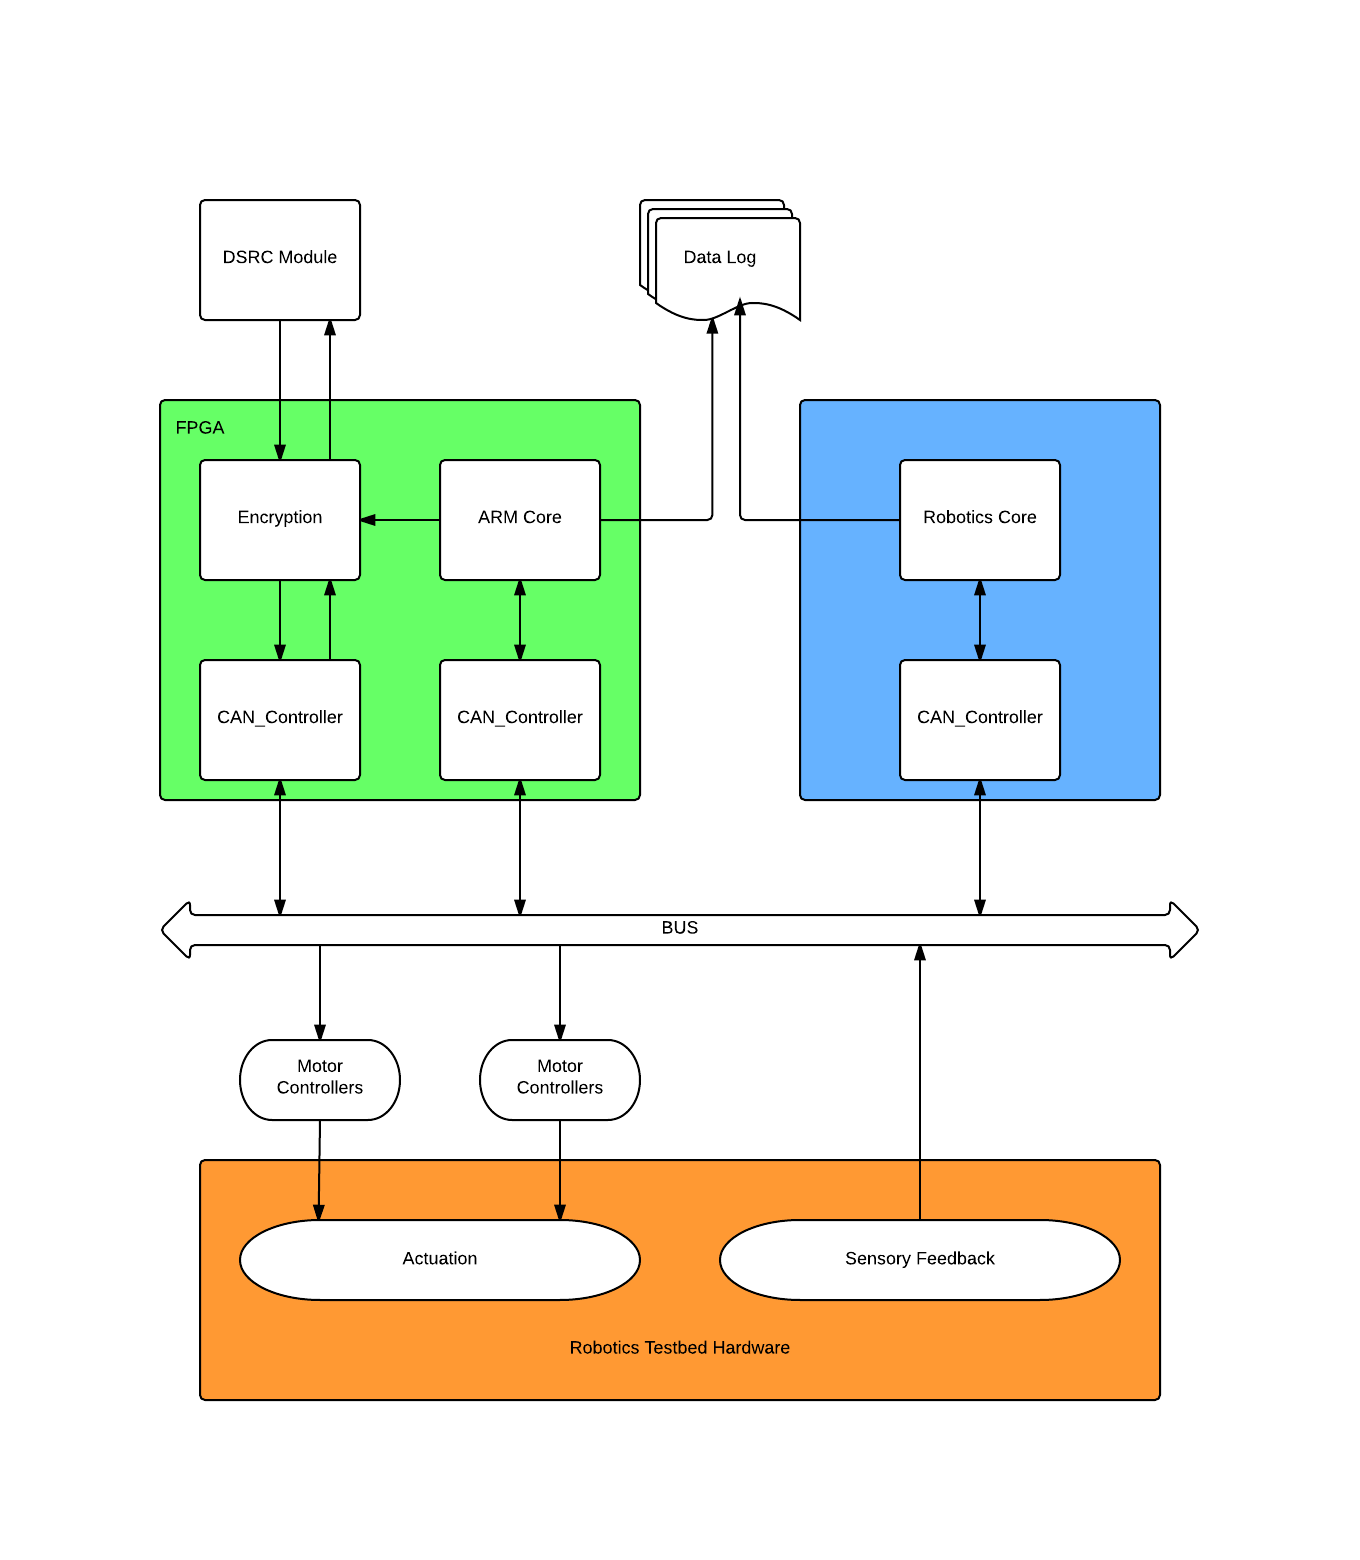
\includegraphics[width = \textwidth]{images/Bus_Layout}
\end{center}

%%% End document
\end{document}